\chapter{Tinjauan Pustaka}

Pada bab ini berisi hasil tinjauan pustaka yang menjadi dasar analisa dan perancangan pada BAB III.
Bab ini secara garis besar berisi keamanan perangkat lunak dan pengujiannya,
tantangan pada pengujian perangkat lunak berbasis web, \emph{Domain-Specific Language}, serta BDD dan TDD.

% \begin{enumerate}
%     \item menunjukkan kepada pembaca adanya gap seperti pada rumusan masalah yang memang belum terselesaikan,
%     \item memberikan pemahaman yang secukupnya kepada pembaca tentang teori atau pekerjaan terkait yang terkait langsung dengan penyelesaian persoalan, serta
%     \item menyampaikan informasi apa saja yang sudah ditulis/dilaporkan oleh pihak lain (peneliti/Tugas Akhir/Tesis) tentang hasil penelitian/pekerjaan mereka yang sama atau mirip kaitannya dengan persoalan tugas akhir.
% \end{enumerate}

% \section{Dasar Teori}
%     \subsection{Subbab}
%     \begin{figure}[h]
%         \centering
%         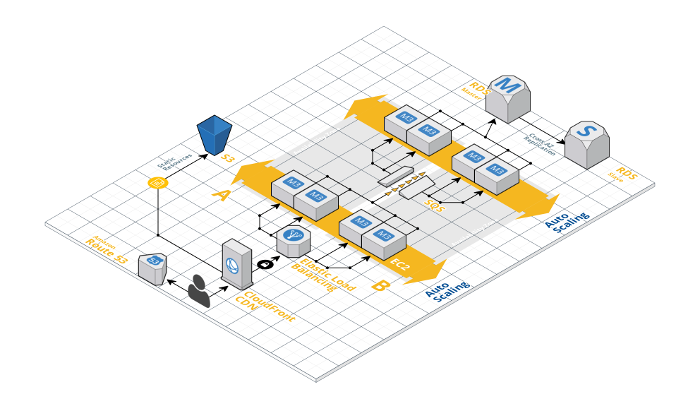
\includegraphics[width=0.8\textwidth]{resources/chapter-2-infrastructure-diagram.png}
%         \caption{Contoh gambar}
%     \end{figure}

\section{Keamanan Perangkat Lunak}

Penggunaan komputer yang semakin hari semakin luas membuat perangkat lunak yang ada semakin besar dan rumit,
yang berarti juga bertambahnya masalah keamanan yang ada pada perangkat lunak tersebut.
Hal ini menyebabkan keamanan perangkat lunak menjadi hal yang semakin penting.

Keamanan perangkat lunak (\emph{software security}) adalah kriteria dimana perangkat lunak tetap bekerja dengan benar
walaupun diserang dengan niat jahat. \emph{Security} berbeda dengan \emph{safety} dimana security fokus terhadap kebenaran
perangkat lunak saat sedang dalam serangan yang dilakukan dengan sengaja, sedangkan \emph{safety} fokus terhadap
kebenaran perangkat lunak saat terjadi kegagalan baik pada tingkat perangkat lunak maupun perangkat keras.

Masalah keamanan perangkat lunak terjadi karena adanya celah atau kecacatan pada perangkat lunak yang dapat
dimanfaatkan oleh penyerang. Celah ini dapat berbentuk kekurangan bawaan pada bahasa pemrograman yang digunakan,
seperti penggunaan \texttt{gets()} pada bahasa C/C++ yang memiliki resiko \emph{buffer overflow},
hingga celah yang terjadi
karena kesalahan pada desain perangkat lunak tersebut. Skala pembuatan perangkat lunak yang semakin besar
dengan proses pengembangan yang melibatkan banyak orang menyebabkan tidak ada satu orang yang paham
cara kerja perangkat lunak secara keseluruhan.

Ada beberapa cara yang dapat dilakukan untuk menanggulangi masalah keamanan perangkat lunak,
namun pada saat ini perlindungan keamanan perangkat lunak dilakukan secara \emph{de facto},
yaitu dengan perlindungan yang diimplementasi setelah aplikasi selesai dikembangkan.
Perlindungan ini biasanya melindungi aplikasi dengan cara memperhatikan data yang masuk
ke dalam aplikasi tidak menimbulkan bahaya atau dapat menyebabkan masalah, pada dasarnya,
perlindungan jenis ini berdasar terhadap pencarian dan mengatasi celah pada aplikasi setelah ditemukan.
Namun, perlindungan perangkat lunak seharusnya mengidentifikasi dan mengatasi masalah dari
dalam perangkat lunak tersebut, sebagai contoh, walaupun ada baiknya mencoba menghadapi serangan
\emph{buffer overflow} dengan membaca \emph{traffic} yang masuk ke dalam aplikasi,
cara yang lebih bagus tentu saja memperbaiki perangkat lunak dari kodenya sehingga
tidak ada kemungkinan \emph{buffer overflow}.

\section{Pengujian Keamanan Perangkat Lunak}

Celah-celah keamanan yang ada pada perangkat lunak selalu menjadi risiko keamanan (\emph{security risk}).
Mengelola risiko keamanan ini menjadi seminimal mungkin adalah salah satu tugas praktisi keamanan perangkat lunak.
Dalam mengelola risiko ini dilakukan beberapa hal, diantaranya:

\begin{itemize}
    \item Membuat kasus penyalahgunaan
    \item Membuat daftar kebutuhan keamanan
    \item Melakukan analisis risiko arsitektur
    \item Membuat perencanaan pengujian keamanan berbasis risiko
    \item Melakukan pengujian keamanan
    \item Melakukan pembersihan setelah terjadinya pelanggaran keamanan
\end{itemize}

Sistem keamanan bukanlah keamanan sistem. Walaupun fitur keamanan seperti \emph{cryptography},
\emph{access control}, dan lain lain memiliki peran penting dalam keamanan perangkat lunak,
keamanan itu sendiri adalah sifat dari sistem secara keseluruhan, bukan hanya dari mekanisme
dan fitur keamanannya. Sebuah \emph{buffer overflow} adalah masalah keamanan, baik itu terletak di dalam
fitur keamanan ataupun di dalam sebuah tampilan non-kritikal.
Karena itu dalam menguji keamanan perangkat lunak memiliki dua macam pendekatan:

\begin{enumerate}
    \item Menguji mekanisme keamanan untuk memastikan bahwa fungsionalitasnya telah diterapkan dengan baik
    \item Melakukan pengujian keamanan berbasis risiko berdasarkan pemahaman dan menyimulasikan pendekatan si penyerang sistem
\end{enumerate}

Banyak \emph{programmer} yang dengan salah mengira bahwa keamanan cukup hanya dengan mengimplementasikan dan
menggunakan fitur-fitur keamanan. Banyak penguji perangkat lunak yang ditugaskan untuk melakukan
pengujian keamanan melakukan kesalahan ini.

Seperti dalam pengujian lainnya, pengujian keamanan perangkat lunak terdiri dari memilih
siapa orang yang akan melakukan pengujian dan apa yang akan dilakukannya.
Dalam memilih orang ada dua kasus tergantung approach yang telah disebutkan,
pada kasus pertama dapat dilakukan oleh staff QA dengan cara pengujian
perangkat lunak seperti biasa untuk melakukan pengujian fungsional
fitur-fitur keamanan sesuai spesifikasi.
Namun pada kasus kedua, staff QA biasa akan kesulitan melaksanakan pengujian berbasis risiko
karena membutuhkan bidang keahlian tertentu.
Pertama, penguji harus dapat berpikir seperti penyerang sistem,
kedua, pengujian keamanan kadang tidak memberikan hasil yang berhubungan langsung dengan
celah keamanan yang ada, sehingga butuh keahlian untuk menginterpretasi dan memahami hasil pengujian.

Kedua, dalam memilih metode pengujian, ada dua metode yang dapat dilakukan.
Pertama dengan cara \emph{White-box} yang dilakukan dengan menganalisis dan memahami
kode serta desain dari program.
Cara ini cukup efektif dalam menemukan kesalahan pemrograman,
dalam beberapa kasus, pengujian ini dapat dilakukan oleh \emph{static analyzer}.
Cara kedua adalah pengujian \emph{Black-box} yang dilakukan dengan cara menguji program
yang sedang berjalan dengan berbagai macam masukan tanpa harus mengetahui masukan program.
Dalam pengujian keamanan, masukan buruk dapat dimasukkan dalam usaha untuk merusak program.
Kedua cara pengujian dapat mengungkapkan adanya risiko keamanan dan kemungkinan eksploitasi.
Masalah yang biasa terjadi dengan pengujian keamanan adalah terkadang organisasi atau perusahaan
tidak memiliki waktu dan sumberdaya untuk melakukan pengujian yang cukup.

Dalam melakukan pengujian keamanan, ada beberapa tantangan yang mungkin dihadapi:
\begin{enumerate}
    \item Adanya efek samping
    
    Dalam melakukan pengujian keamanan dengan pendekatan menguji fungsionalitas perangkat lunak,
    biasanya diberikan sebuah masukan A dan diperiksa apakah perangkat lunak mengembalikan
    hasil B sesuai dengan spesifikasi.
    Namun yang kadang terlupakan bahwa aplikasi dapat memiliki efek samping yang dapat dimanfaatkan
    penyerang sebagai celah keamanan. Salah satu contohnya adalah perangkat utilitas 
    RDISK pada Windows NT 4.0,  yang berfungsi untuk membuat \emph{Emergency Repair Disk}.
    Program ini pada umumnya berjalan baik sesuai spesifikasi, namun saat program berjalan,
    ia membuat sebuah file sementara yang dapat dibaca oleh siapa saja.
    Hal ini berarti pengguna tamu (\emph{guest}) dapat membaca isi file tersebut yang
    termasuk \emph{registry Windows} yang berisi pengaturan tentang sistem yang dapat dimanfaatkan penyerang.

    \item Keadaan Pengujian Keamanan Saat Ini

    Perusahaan yang menyediakan jasa pengujian keamanan biasanya memiliki daftar-daftar celah yang umum ada.
    Mereka biasanya hanya menggunakan daftar tersebut untuk membuat rencana pengujian.
    Cara seperti ini biasanya tidak akan dapat menemukan celah-celah keamanan yang baru.

    \item Ketidakamanan dan kegagalan aplikasi penunjang

    Perangkat lunak modern berjalan pada sistem yang saling bergantung satu sama lain,
    dimana satu aplikasi menggunakan puluhan \emph{library} dan berkomunikasi dengan
    beberapa komponen lainnya.
    Hal ini dapat menimbulkan dua masalah.
    Pertama, aplikasi dapat memiliki celah dari salah satu komponen yang ia gunakan.
    Kedua, sebuah komponen yang digunakan untuk menyediakan fungsionalitas keamanan
    dapat saja pada suatu saat rusak dan berhenti bekerja.

    \item Masukan tidak terkira dari pengguna

    Masukan dari pengguna adalah salah satu sumber celah yang paling umum dan paling mudah dieksploitasi.
    Beberapa contoh yang umum digunakan adalah masukan yang panjang, karakter spesial, dan nilai-nilai khusus.
    Salah satu contoh celah yang terjadi dari masukan pengguna ini adalah \emph{buffer overflow},
    yang memungkinkan penyerang menyisipkan kode pada masukan yang sangat panjang,
    hingga tidak bisa ditampung \emph{buffer} dan dijalankan oleh komputer. 

    \item Ketidakamanan desain

    Banyak celah keamanan terjadi sejak perangkat lunak masih dalam tahap desain.
    Kadang celah tersebut tidak bisa langsung diketahui karena terjadi setelah semua
    bagian sistem selesai dirancang namun gabungan dari keseluruhan sistem tersebut
    menyebabkan adanya celah.
    Kadang celah juga terjadi pada test interface, yaitu bagian program yang sengaja
    disisipkan dan memberi celah untuk pengujian, namun tidak dihilangkan saat program akan dirilis.

    \item Ketidakamanan implementasi

    Walaupun spesifikasi perangkat lunak telah didesain sebaik mungkin dengan
    mempertimbangkan berbagai macam aspek keamanan,
    celah tetap dapat terjadi karena implementasi perangkat lunak yang tidak sempurna.

\end{enumerate}

\section{Tantangan Dalam Pengujian Aplikasi \emph{Web}}

Perangkat lunak berbasis web adalah salah satu jenis perangkat lunak paling umum pada saat ini.
Perangkat lunak ini menjadi tulang belakang dari komunikasi di dunia dan banyak hal-hal
yang membutuhkan keamanan tinggi menggunakan perangkat lunak berbasis web seperti perbankan.
Hal seperti menyebabkan perangkat lunak berbasis web menjadi salah satu target yang empuk untuk
dimanfaatkan celah dan kekurangannya. Sifat dari aplikasi web yang dinamis, kompleks, dan
selalu berubah-ubah membuat semakin mudahnya muncul celah baru pada aplikasi web jika tidak diperhatikan.

Beberapa masalah umum yang ada pada perangkat lunak berbasis web adalah:
\begin{enumerate}
    \item Autentikasi: memastikan pengguna yang meminta data adalah benar pengguna tersebut
    \item Autorisasi: memastikan pengguna boleh melakukan hal yang dilakukannya.

    \item \emph{Cross-site scripting}:
    celah dimana penyerang dapat memasukkan kode jahat ke halaman web yang dijalankan di browser pengguna lain.

    \item \emph{SQL injection}:
    celah dimana disisipkannya kode jahat di dalam perintah SQL yang kemudian dijalankan oleh \emph{database}.

    \item \emph{Cross-site request forgery}:
    celah dimana sebuah \emph{website} dapat dieksploitasi untuk mengirimkan perintah palsu dari sebuah user.

    \item \emph{Malicious file execution}:
    aplikasi web menjalankan kode jahat yang berada di sebuah file bebas
\end{enumerate}

Beberapa tantangan dalam melakukan pengujian keamanan terhadap aplikasi web adalah:
\begin{enumerate}
    \item Butuhnya pengembangan kakas yang dapat mengotomatisasi pengujian aplikasi web.
    
    \item Pengembangan aplikasi web yang dinamis dan \emph{Rich Content} seperti \emph{Single-Page Application}
    mempersulit \emph{crawling} halaman web sehingga bisa saja ada state halaman yang
    tidak bisa dicapai oleh kakas pengujian.

    \item Bahasa pemrograman yang digunakan pada implementasi tidak memiliki fitur yang
    dapat memaksa penggunaan aturan keamanan yang dapat menyebabkan bahaya terhadap keamanan
    dan integritas data pengguna.
\end{enumerate}

\section{\emph{Domain-Specific Language}}

\emph{Domain-Specific Language} (DSL) adalah bahasa pemrograman berkemampuan terbatas yang
berfokus pada suatu domain tertentu.

Dari definisi diatas, ada empat poin penting:

\begin{enumerate}
    \item DSL dapat digunakan untuk memerintahkan komputer. Seperti bahasa pemrograman lainnya,
    DSL haruslah bisa untuk dipahami manusia, tetapi masih mungkin diolah oleh komputer.

    \item DSL adalah bahasa pemrograman komputer. Hal ini berarti DSL harus terasa seperti
    bahasa yang dimana kemampuannya tidak hanya muncul dari masing-masing ekspresinya,
    tetapi juga saat ekspresi-ekspresi tersebut digabungkan.

    \item Bahasa pemrograman umum (\emph{General Purpose Programming Language}) memiliki banyak fitur.
    Hal ini membuatnya sangat berguna, namun menjadi susah untuk dipelajari dan digunakan.
    DSL dengan kemampuannya yang terbatas hanya memiliki fitur-fitur minimum yang dibutuhkan untuk domainnya.

    \item Sebuah bahasa dengan kemampuan terbatas hanya akan berguna jika ia memiliki
    fokus yang jelas terhadap sebuah domain kecil.
\end{enumerate}

DSL terbagi menjadi dua kategori, yaitu:

\begin{enumerate}
    \item \emph{External DSL}

    DSL eksternal adalah bahasa yang terpisah dari bahasa utama aplikasi.
    Biasanya, DSL eksternal memiliki syntaxnya sendiri, namun kadang dapat menggunakan
    bahasa lain seperti XML. Sebuah kode pada DSL eksternal biasanya akan diproses oleh
    aplikasi utama. Beberapa contoh DSL eksternal adalah Regex, SQL, awk, sed.

    \item \emph{Internal DSL}
    
    DSL internal adalah sebuah cara tertentu untuk menggunakan sebuah bahasa.
    Sebuah DSL internal ditulis dalam bahasa yang sama dengan bahasa utama aplikasi,
    namun hanya menggunakan sebagian fitur bahasa untuk mengurusi bagian kecil 
    dari keseluruhan sistem. Salah satu bahasa yang memiliki banyak DSL internal adalah Ruby,
    karena struktur Ruby yang ekspresif memudahkan dibuatnya DSL.
    Web framework Rails yang ditulis dengan Ruby adalah salah satu contoh DSL.
\end{enumerate}

DSL adalah sebuah alat yang memiliki fokus yang jelas dan hanya mengurusi suatu
aspek kecil tertentu. Sebuah aplikasi bisa saja menggunakan banyak DSL untuk mengurusi
berbagai aspek sistemnya. Beberapa kelebihan menggunakan DSL adalah:

\begin{enumerate}
    \item Meningkatkan produktivitas

    Salah satu daya tarik utama dari DSL adalah ia menyediakan cara untuk menyampaikan
    sebuah maksud sebuah sistem dengan lebih jelas.
    Hal ini menyebabkan programmer lebih mudah memahami maksud dan
    tujuan sebuah kode dan sistem.

    \item Merepresentasikan pengetahuan domain dengan lebih baik

    DSL dapat didesain sedemikian mungkin untuk merepresentasikan dan mengabstraksikan
    suatu domain tertentu, sehingga
    bisa digunakan bukan hanya oleh \emph{programmer} saja, tetapi juga oleh ahli domain tersebut.
\end{enumerate}

Sementara kekurangan menggunakan DSL adalah:

\begin{enumerate}
    \item \emph{Language cacophony}
    
    Beberapa komplain yang sering didengar saat menggunakan DSL adalah \emph{language cacophony},
    dimana bahasa biasanya sulit untuk dipelajari, sehingga menggunakan banyak bahasa akan lebih
    sulit dari pada menggunakan satu bahasa. Kebutuhuan untuk mempelajari banyak bahasa menyebabkan
    sulit untuk mengerjakan proyek dan menambah orang baru kedalam proyek.

    Namun dari komplain ini, banyak orang yang berpikiran bahwa mempelajari sebuah DSL akan sesulit
    mempelajari bahasa pemrograman general biasa. Tetapi, DSL sebenarnya lebih mudah dipelajari
    karena keterbatasannya.

    \item Biaya pembuatan
    
    Seperti semua bagian dari program, DSL juga merupakan program yang harus dibuat dan dipelihara.
    Tentu saja hal ini dapat menambah biaya yang harus dikeluarkan. Biaya pembuatan DSL juga dapat
    lebih tinggi karena tim yang ada tidak terbiasa membuat DSL sehingga harus belajar lagi, yang
    juga dapat menambah biaya.

\end{enumerate}

% TODO: BDD Testing and Gherkin